\usetikzlibrary{arrows.meta}
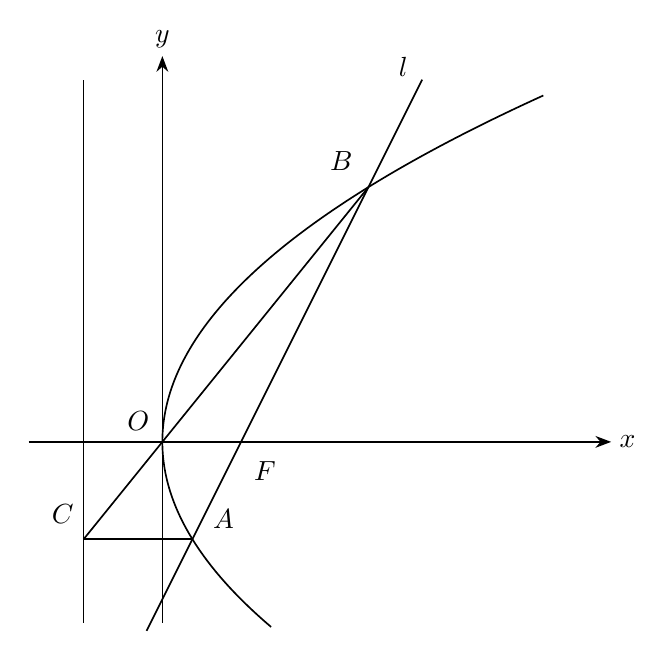
\begin{tikzpicture}[x=1cm,y=1cm,line width=.6pt,font=\normalsize,>=Stealth,
  axis/.style={->,line width=.6pt},curve/.style={line width=.6pt},segment/.style={line width=.6pt},label/.style={inner sep=1pt}]
\def\pp{2}
\coordinate (O) at (0.0,0.0);
\coordinate (F) at (1.0,0.0);
\coordinate (A) at (0.381966,-1.236068);
\coordinate (B) at (2.618034,3.236068);
\coordinate (C) at (-1.0,-1.236068);
\coordinate (L1) at (-0.2,-2.4);
\coordinate (L2) at (3.3,4.6);
\coordinate (X1) at (-1.0,-2.3);
\coordinate (X2) at (-1.0,4.6);
\coordinate (AX1) at (-1.7,0.0);
\coordinate (AX2) at (5.7,0.0);
\coordinate (AY1) at (0.0,-2.3);
\coordinate (AY2) at (0.0,4.9);
\draw[axis] (AX1)--(AX2);
\draw[axis] (AY1)--(AY2);
\draw[curve] plot[domain=-2.35:4.4,samples=180,variable=\t] ({(\t*\t)/(2*\pp)},{\t});
\draw[segment] (X1)--(X2);
\draw[segment] (L1)--(L2);
\draw[segment] (C)--(A);
\draw[segment] (C)--(B);
\node[label,anchor=south east] at (-0.12,0.1) {$O$};
\node[label,anchor=north west] at (1.12,-0.2) {$F$};
\node[label,anchor=south west] at (0.6,-1.14) {$A$};
\node[label,anchor=south east] at (2.46,3.4) {$B$};
\node[label,anchor=south east] at (-1.08,-1.08) {$C$};
\node[label,anchor=south east] at (3.16,4.6) {$l$};
\node[label,anchor=west] at (5.76,0.0) {$x$};
\node[label,anchor=south] at (0.0,4.96) {$y$};
\end{tikzpicture}
